{\sihao \kaishu 参照以下提纲撰写,要求内容翔实、清晰,层次分明,标题突出。{\color{MsBlue} \bfseries 请勿删除或改动下述提纲标题及括号中的文字。}}
\vskip -5mm
{\color{MsBlue} \subsection{\texorpdfstring{\sihao \kaishu \quad \ (一)立项依据与研究内容\textnormal{\kaishu (建议8000字以内):}}{(一)立项依据与研究内容(建议8000字以内):}}}

%------------------------ 以下是本部分具体内容 ------------------

% 注意:这里暂时不要用 \currfiledir 拼接路径,
% 因为统计字数工具 texcount 无法处理带变量的路径,它不会把 \currfiledir 替换成实际路径

%------------------------ 项目的立项依据 -----------------------
% 未完成

% \input{\currfiledir 1-项目的立项依据}
{\sihao \kaishu \color{MsBlue} 1.{\bfseries 项目的立项依据}(研究意义、国内外研究现状及发展动态分析,需结合科学研究发展趋势来论述科学意义;或结合国民经济和社会发展中迫切需要解决的关键科技问题来论述其应用前景。附主要参考文献目录);}

\vskip 2mm
\subsubsection{\bfseries 研究意义:}
% 未完成

待写。。。。


\subsubsection{\bfseries 国内外研究现状:}
% 未完成

待写。。。。


\subsubsection{\bfseries 发展动态分析:}
% 未完成

待写。。。。


\ifhandout
% do nothing
\else
\begin{center}
{\larger[2]\color{red} \ding{43}\ding{43} 立项依据部分共计 \wordcount 字 \reflectbox{\ding{43}\ding{43}}}
\end{center}
\fi


\vskip 5mm


%-------------------- 参考文献 -------------------

% 采用 GB/T 7714 (numerical) 样式以支持中文文献,这样做的另外一个优点是该包兼容natbib,修改参考文献的行距也比较方便,缩短了一些。如有需要,也可以切换回之前版本用的ieeetrNSFC
%\newpage
%\bibliographystyle{ieeetrNSFC}
% \bibliographystyle{gbt7714-numerical}
% \bibliography{references}
\printbibliography[title=参考文献]
\newpage


%---------- 项目的研究内容、研究目标、拟解决的关键科学问题 -----------
% 未完成

% \input{\currfiledir 2-项目的研究内容-研究目标-以及拟解决的关键科学问题}
{\sihao \color{MsBlue} \kaishu 2. {\bfseries 项目的研究内容、研究目标,以及拟解决的关键科学问题}(此部分为重点阐述内容);}

\subsubsection{\bfseries 2.1 研究内容:}
% 未完成

\noindent{\bfseries 研究内容 1:}

\noindent{\bfseries 研究内容 2:}

\noindent{\bfseries 研究内容 3:}

见\cref{fig:sample-tikz}。

\begin{figure}[!htp]
\centering
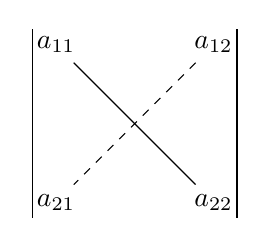
\begin{tikzpicture}
\node at (0,2) (a11) {$a_{11}$};
\node at (2,2) (a12) {$a_{12}$};
\node at (0,0) (a21) {$a_{21}$};
\node at (2,0) (a22) {$a_{22}$};
\draw (-0.3, 2.2) -- (-0.3, -0.2);
\draw (2.3, 2.2) -- (2.3, -0.2);
\draw (a11) -- (a22);
\draw[dashed] (a12) -- (a21);
\end{tikzpicture}
\caption{Tikz示例图}
\label{fig:sample-tikz}
\end{figure}


见\cref{fig:sample-fig}。

\begin{figure}[!htp]
\centering
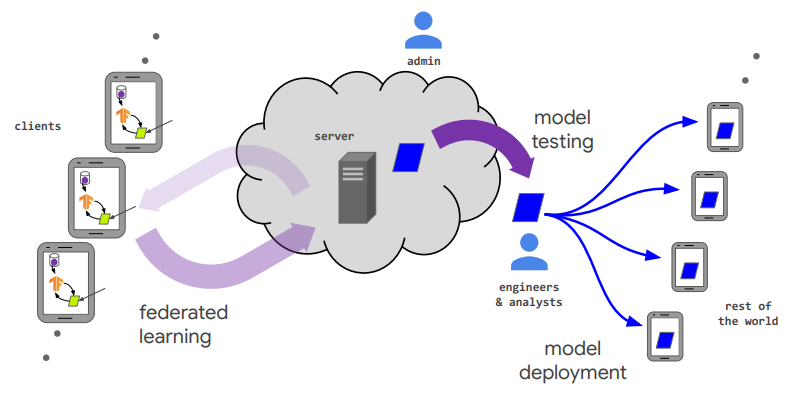
\includegraphics[width=0.75\textwidth]{figures/sample-fig.png}
\caption{示例图}
\label{fig:sample-fig}
\end{figure}


\subsubsection{\bfseries 2.2 研究目标:}
% 未完成

本项目针对待写。。。。


\subsubsection{\bfseries 2.3 关键问题:}
% 未完成

待写。。。。


\ifhandout
% do nothing
\else
\begin{center}
{\larger[2]\color{red} \ding{43}\ding{43} 研究内容部分共计 \wordcount 字 \reflectbox{\ding{43}\ding{43}}}
\end{center}
\fi


\vskip 5mm


%---------------------- 研究方案及可行性分析 --------------------
% 未完成

% \input{\currfiledir 3-拟采取的研究方案及可行性分析}
{\sihao \color{MsBlue} \kaishu 3.{\bfseries 拟采取的研究方案及可行性分析}(包括研究方法、技术路线、实验手段、关键技术等说明);}

\subsubsection{{\bfseries 拟采取的研究方案:}}
% 未完成

待写。。。。


\subsubsection{{\bfseries 可行性分析:}}
% 未完成

待写。。。。


\ifhandout
% do nothing
\else
\begin{center}
{\larger[2]\color{red} \ding{43}\ding{43} 研究方案部分共计 \wordcount 字 \reflectbox{\ding{43}\ding{43}}}
\end{center}
\fi


\vskip 5mm


%--------------------- 本项目的特色与创新之处 --------------------
% 未完成

% \input{\currfiledir 4-本项目的特色与创新之处}
{\sihao \color{MsBlue} \kaishu 4.{\bfseries 本项目的特色与创新之处;}}

\subsubsection{{\bfseries 项目特色:}}
% 未完成

待写。。。。


\subsubsection{{\bfseries 项目创新:}}
% 未完成

待写。。。。


\ifhandout
% do nothing
\else
\begin{center}
{\larger[2]\color{red} \ding{43}\ding{43} 特色创新部分共计 \wordcount 字 \reflectbox{\ding{43}\ding{43}}}
\end{center}
\fi


\vskip 5mm


%------------------- 年度研究计划及预期研究结果 -------------------
% 未完成

% \input{\currfiledir 5-年度研究计划及预期研究结果}
{\sihao \color{MsBlue} \kaishu 5.{\bfseries 年度研究计划及预期研究结果}(包括拟组织的重要学术交流活动、国际合作与交流计划等)。}

\subsubsection{{\bfseries 年度研究计划:}}
% 未完成

\uline{\bfseries 2025年度}:

待写。。。。

\uline{\bfseries 2026年度}:

待写。。。。

\uline{\bfseries 2027年度}:

待写。。。。

\uline{\bfseries 2028年度}:

待写。。。。


\subsubsection{{\bfseries 预期研究结果:}}
% 未完成

通过四年的努力,力争。。。。


\ifhandout
% do nothing
\else
\begin{center}
{\larger[2]\color{red} \ding{43}\ding{43} 研究计划部分共计 \wordcount 字 \reflectbox{\ding{43}\ding{43}}}
\end{center}
\fi


\vskip 5mm



\ifhandout
% do nothing
\else
\begin{center}
{\larger[2]\color{red} \ding{43}\ding{43} 立项依据与研究内容部分共计 \wordcount 字 \reflectbox{\ding{43}\ding{43}}}
\end{center}
\fi
